\subsection{Описание кода программной реализации}
Код реализации выложен на \mintinline{bash}{C++} в репозитории \cite{Repository}. Диаграмма калссов реализации представлена на рисунке \ref{fig:UML}.

\begin{figure}[!htbp]
    \centering
    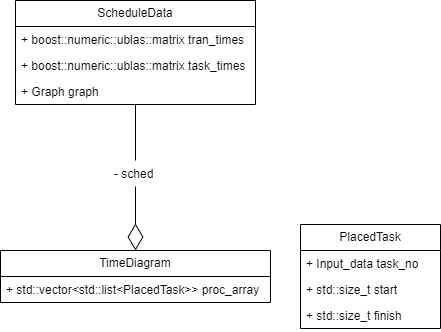
\includegraphics[width=0.8\textwidth]{imgs/final_UML.drawio.png}
    \caption{UML-диаграмма реализации}
    \label{fig:UML}
\end{figure}

Среди представленных классов:
\begin{itemize}
    \item \mintinline{C++}{ScheduleData} - класс, хранящий в себе входные данные и выполняющий всю необходимую их предобработку.
    \item \mintinline{C++}{TimeDiagram} - класс, хранящий в себе частичное или полное расписание.
    \item \mintinline{C++}{PlacedTask} - класс, хранящий в себе информацию о поставленной в расписание работе.
\end{itemize}

Жадные алгоритмы реализованы в функциях, не инкапсулированных в классах:
\begin{itemize}
    \item \mintinline{C++}{construct_time_schedule()} - жадный алгоритм с жадным критерием.
    \item \mintinline{C++}{greedy_EDF_heuristic()} - Жадный алгоритм с EDF эвристикой.
\end{itemize}

В репозиторий включены следубщие библиотеки:
\begin{enumerate}
    \item \mintinline{bash}{METIS} 5.1.0 \cite{METIS_lib} - библиотека для разбиения графов.
    \item \mintinline{bash}{json} 3.11.2 \cite{json_lib} - библиотека для работы с форматом JSON. Используется для составления выходных файлов.
    \item \mintinline{bash}{toml11} 3.7.1 \cite{toml11_lib} - библиотека для работы с форматом TOML. Используется для чтения конфигурационных файлов.
\end{enumerate}

Также, у реализации есть зависимость, не включенная в репозиторий - \mintinline{bash}{boost} 1.80 \cite{boost_framework}. Для сборки проекта используется \mintinline{bash}{CMake}. Инструкция по сборке приведена в листинге \ref{lst:build}. Для сборки документации (на английском) используется \mintinline{bash}{Doxygen}. Инфструкция по сборке документации приведена в листинге \ref{lst:docs}

\begin{listing}[!htbp]
    \begin{minted}{bash}
        mkdir build
        cd build
        cmake ..
        make
    \end{minted}
    \caption{Сборка программной реализации}
    \label{lst:build}
\end{listing}

\begin{listing}[!htbp]
    \begin{minted}{bash}
        doxygen Doxyfile
    \end{minted}
    \caption{Сборка документации}
    \label{lst:docs}
\end{listing}


\subsection{Описание интерфейса программной реализации}
\subsubsection{Параметры командной строки}
Из исходного кода реализации алгоритма собираетяс утилита, с интерфейсом, описанным в листинге \ref{lst:template} и таблице \ref{tbl:command-line-parameters}. 
\begin{listing}[!htbp]
    \begin{minted}[breaklines]{bash}
        opts <algorithm_name> --input <input_file> --output <output_file> --conf <config_file> --log <log_level>
    \end{minted}
    \caption{Шаблон запуска утилиты построения расписания}
    \label{lst:template}
\end{listing}

\begin{table}[!htbp]
    \centering
    \begin{tabularx}{\textwidth}{|c|X|}
        \hline
        Имя                      & Описание                                     \\
        \hline
        \texttt{algorithm\_name} & Название алгоритма для построения расписания \\
        \hline
        \texttt{input}           & Путь к файлу с входными данными              \\
        \hline
        \texttt{output}          & Путь к файлу с выходными данными             \\
        \hline
        \texttt{conf}            & Путь к файлу с конфигурацией                 \\
        \hline
        \texttt{log}             & Уровень логирования                          \\
        \hline
    \end{tabularx}
    \caption{Параметры командной строки программы}
    \label{tbl:command-line-parameters}
\end{table}
\subsubsection{Описание конфигурационных файлов}
В качестве формата конфигурационных файлов был выбран формат \texttt{toml}. Пример конфигурационного файла приведен в листинге \ref{lst:config-file} и таблице \ref{tbl:config-file-parameters}. Конфигурационный файл содержит два раздела:
\begin{itemize}
    \item Раздел \texttt{[general]}, отвечающий за общие параметры построения расписания.
    \item Раздел \texttt{[greedy]}, отвечающий за параметры, относящиеся только к жадному алгоритму.
\end{itemize}

\begin{table}[!htbp]
    \centering
    \begin{tabularx}{\textwidth}{|c|X|}
        \hline
        Поле                & Описание                                                                                                                                      \\
        \hline
        \texttt{criteria}   & Критерий, дополнительное ограничение котрого будет выполняться (CR / NO)                                                                      \\
        \hline
        \texttt{CR\_bound}  & Верхняя граница ограничения $CR$ (если используется)                                                                                          \\
        \hline
        \texttt{inp\_class} & Класс типа входных данных
        \begin{itemize}
            \item \texttt{class\_1} для постановки с однородными процессорами
            \item \texttt{class\_general} для постановки с неоднородными процессорами
        \end{itemize}                                                                                            \\
        \hline
        \texttt{cr\_con}    & Переключение жадного критерия в жадном алгоритме с жадными критериями с максимального количества потомков на максимальное количество предков. \\
        \hline
    \end{tabularx}
    \caption{Параметры конфигурационного файла.}
    \label{tbl:config-file-parameters}
\end{table}
\begin{listing}
    \begin{minted}[linenos]{toml}
        [general] 
        criteria = "BF" 
        CR_bound = 0.4 
        inp_class = "class_1" 
        
        [greedy] 
        cr_con = false
    \end{minted}
    \caption{Пример конфигурационного файла}
    \label{lst:config-file}
\end{listing}

\subsubsection{Описание выходных файлов}
В качестве формата выходных файлов был выбран формат \texttt{json}. Пример конфигурационного файла приведен \ref{lst:output-file} и таблице \ref{tbl:output-file-fields}. Конфигурационный файл содержит информацию о характеристиках построенного расписания, а так же информацию о привзяках и порядке постановке работ на процессорах.
\begin{table}[!htbp]
    \centering
    \begin{tabularx}{\textwidth}{|c|X|}
        \hline
        Поле                & Описание                                                                                                                                                \\
        \hline
        \texttt{CR}         & Значение ограничения $CR$ построенного расписания.                                                                                                      \\
        \hline
        \texttt{algo\_time} & Время выполнения алгоритма, в миллисекундах                                                                                                             \\
        \hline
        \texttt{criteria}   & Дополнительное ограничение, используемое для построения рапсисания                                                                                      \\
        \hline
        \texttt{nodes}      & Количество работ во входном графе.                                                                                                                      \\
        \hline
        \texttt{time}       & Время выполнения построенного расписания                                                                                                                \\
        \hline
        \texttt{procs}      & Словарь с номерами процессоров в качестве ключей и массивами постанленных на соответствующий процессор работами. Каждая поставленная работа состоит из:
        \begin{itemize}
            \item \texttt{task\_dur} - время выполнения работы на поставленный процессор.
            \item \texttt{task\_no} - идентификатор работы.
            \item \texttt{task\_start} - время начала выполнения работы на процессоре.
        \end{itemize}                                                                                                  \\
        \hline
    \end{tabularx}
    \caption{Поля выходного файла}.
    \label{tbl:output-file-fields}
\end{table}

\begin{listing}[!htbp]
    \begin{minted}[linenos, mathescape=true, escapeinside=||]{json}
        {  
            "CR": 0.3221312,  
            "algo_time": 300, 
            "criteria": "CR", 
            "nodes": 2000, 
            "procs": { 
                "0": [ 
                    { 
                        "task_dur": 5, 
                        "task_no": 1202, 
                        "task_start": 0 
                    }, 
                    { 
                        "task_dur": 3, 
                        "task_no": 1608, 
                        "task_start": 5 
                    },
                    |\ldots|
                ], 
                "1": [ 
                    |\ldots|
                ], 
                |\ldots|
            }, 
            "time": 2211 
        }
    \end{minted}
    \caption{Пример выходного файла}
    \label{lst:output-file}
\end{listing}
